\subsubsection{The sinking block benchmark}
\label{sec:sinking_block}

This benchmark is based on the benchmark presented in \cite{gery10} and extended in \cite{thie11}.
It consists of a two-dimensional $512~\si{\km}\times 512~\si{\km}$ domain filled with a fluid (the ``mantle'')
of density $\rho_1=3200\si{\kg\per\cubic\meter}$ and viscosity $\eta_1=10^{21}~\si{\pascal\second}$.
A square block of size $128~\si{\km}\times 128~\si{\km}$ is placed in the domain and is centered at location $(x_c,y_c)=(256~\si{\km},384~\si{\km})$
so as to ensure that its sides align with cell boundaries at all resolutions (GMR level $\geq 3$). It is filled with a fluid of density
$\rho_2=\rho_1+\delta \rho$ and viscosity $\eta_2$. The gravity vector points downwards with
$|\boldsymbol{g}|=10~\si{\meter\per\square\second}$. Boundary conditions are free slip on all sides.
Only one time step is carried out and we measure the absolute velocity $|v_z|$ in the middle of the block.

In a geodynamical context, the block could be interpreted as a detached slab or a plume head.
As such its viscosity and density can vary (a cold slab has a higher effective viscosity than the surrounding mantle while
it is the other way around for a plume head). The block densities can then vary from a few units to several
hundreds of $\si{\kg\per\cubic\meter}$ and the viscosities by several orders of magnitude to represent a wide array of scenarios.
The velocity field obtained for $\eta_2=10^{27}~\si{\pascal\second}$ and $\delta\rho=32~\si{\kg\per\cubic\meter}$ is shown in
Figure~\ref{fig:sinking_block1}.

As shown in \cite{thie11} one can independently vary $\eta_1$, $\rho_2$, $\eta_2$, and measure $|v_z|$ for each combination: the quantity
$|v_z| \eta_1/\delta\rho$ is then found to be a simple function of the ratio $\eta^\star=\eta_1/\eta_2$:
at high enough mesh resolution all data points collapse onto a single line.
The shell script {\sl run\_benchmark} in the folder runs the experiment for values
$\eta_2\in [10^{17},10^{26}]~\si{\pascal\second}$ and $\delta\rho=8,32,128~\si{\kg\per\cubic\meter}$.
Results are shown in Figure~\ref{fig:sinking_block2} and we indeed recover the expected trend with
all data points forming a single smooth line.

\begin{figure}
  \centering
  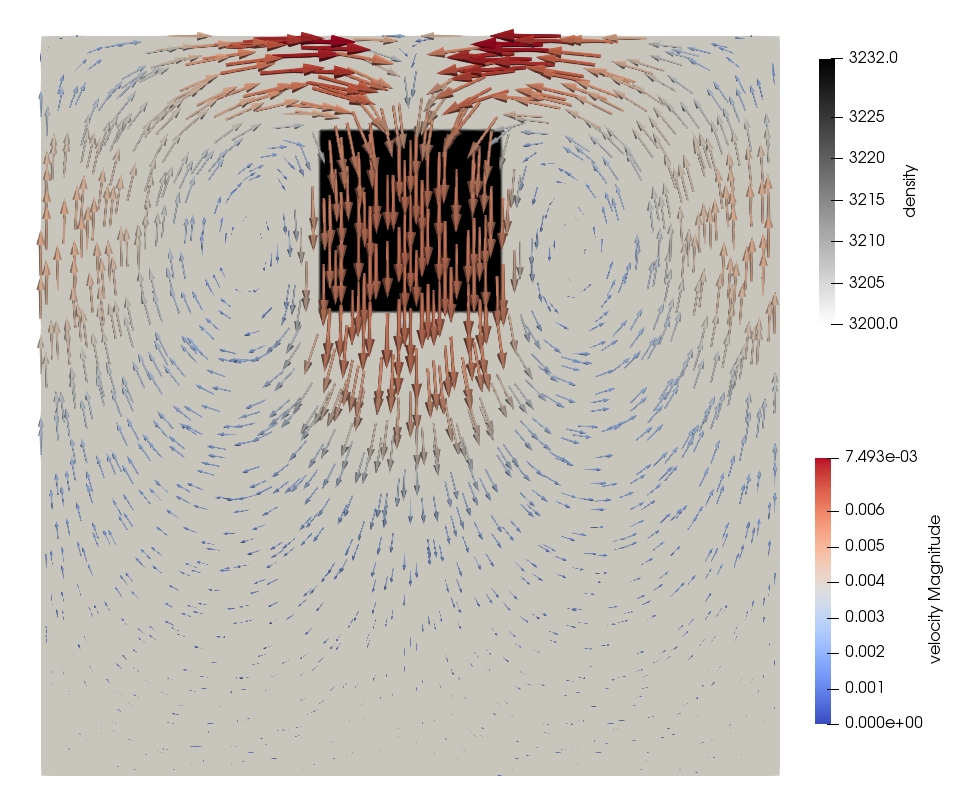
\includegraphics[width=0.6\textwidth]{cookbooks/benchmarks/sinking_block/doc/dens_vel.png}
  \caption{\it Density field with velocity arrows for $\eta_2=10^{27}~\si{\pascal\second}$ and $\delta\rho=32~\si{\kg\per\cubic\meter}$}
  \label{fig:sinking_block1}
\end{figure}

\begin{figure}
  \centering
  \includesvg[width=0.8\textwidth]{cookbooks/benchmarks/sinking_block/doc/plot.svg}
  \caption{\it Scaled velocity measurements as a function of the viscosity contrast between surrounding medium and block for all experiments.}
  \label{fig:sinking_block2}
\end{figure}
